% !TeX spellcheck = es_ES
\documentclass[arial,a4paper,print]{article}

\usepackage{amsmath}
\usepackage{helvet}
\usepackage{lipsum}
\usepackage{multirow}
\usepackage{array}
\usepackage{physics}
\usepackage[version=4]{mhchem}
\usepackage{epsfig}
\usepackage{amssymb}
%\usepackage{svrsymbols}
\usepackage{siunitx}
\usepackage{graphicx}
\usepackage{subcaption}
\usepackage[labelfont=sc, font={footnotesize, singlespacing}]{caption}
\usepackage[margin=2cm]{geometry}  

\renewcommand{\familydefault}{\sfdefault}

\usepackage[spanish]{babel}
%opening
\title{Física: Selectividad 2022}
\author{tomiock}

\begin{document}

\maketitle

\section{Ondas y sonido}
Usualmente este tema se divide en dos, una parte corresponde al MAS y la otra al sonido/ondas estacionarias.
\subsection{Movimiento Armónico Simple}
En la figura \ref{fig:mememhs} se puede ver un meme sobre el Movimiento Armónico Simple.
% TODO:  required
\begin{figure}[h]
	\centering
	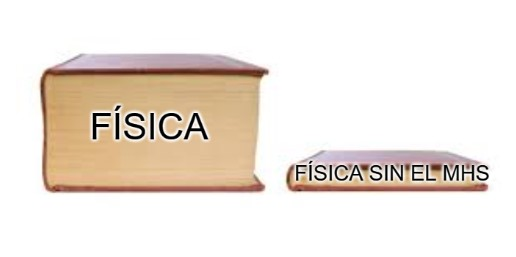
\includegraphics[width=0.3\linewidth]{meme_MHS}
	\caption{Meme totalmente cierto sobre el Movimiento Armónico Simple}
	\label{fig:mememhs}
\end{figure}

Está en todas parte, es la base de las ondas, i por lo tanto del 70\% de la física. Sirve para describir un movimiento cíclico o periódico. Tienen una frecuencia $\nu$, periodo $T$ y velocidad angular $\omega$, que se relacionan como:
\begin{align*}
	&\nu = \frac1T \\
	\omega &= \frac{2\pi}{T} = 2\pi\nu
\end{align*}

Una variable $y$ es descrita por un MAS se expresa como:
\begin{equation*}
	y = A\sin\theta
\end{equation*}

Podemos hacer que el movimiento sea dependiente del tiempo a través de la velocidad angular $\omega$:
\begin{align}
	& \theta(t) = \omega t + \varphi_{0} \\
	\Rightarrow \,& y = A\sin(\omega t + \varphi_{0})
\end{align}

Al derivar la ecuación (2) se pueden obtener la velocidad i al aceleración que describen un MAS, las cuáles también son un MAS pero con la amplitud modificada mediante la regla de la cadena:
\begin{align*}
	 v &= \dv{y}{t} = \omega A \cos(\omega t + \varphi_{0}) \\
	 a &= \dv{v}{t} = \dv[2]{y}{t} = -\omega^{2}A\sin(\omega t + \varphi_{0})
\end{align*}
 Se puede ver como la velocidad máxima es $v_{max} = \omega A$ y la aceleración $a_{max} = \omega^{2}A$.

También tenemos que:
\begin{equation*}
	a = -\omega^{2}y
\end{equation*}
Donde $y$ es el MAS original que describe el movimiento. 

\subsection{Onda plana}
Si describimos un MAS con el espacio y el tiempo tenemos el concepto de onda plana. La cual tiene asociada una velocidad de propagación $v$:
\begin{equation*}
	v=\frac{\lambda}{T} = \lambda\nu
\end{equation*}
Donde $\lambda$ es la longitud de onda. 

Una onda plana se describe como:
\begin{equation*}
	y(x,t) = A \sin\left(\frac{2\pi}{T}t - \frac{2\pi}{\lambda}x + \varphi_{0}\right)
\end{equation*}

Se define un nombre de onda $k=\frac{2\pi}{\lambda}$ que es el número de ciclos que se completan en una distancia $2\pi$ metros.

Por lo tanto tenemos que:
\begin{equation*}
	y(x,t) = A \sin\left(\omega t \pm kx + \varphi_{0}\right)
\end{equation*}
Donde $\omega t \pm kx + \varphi_{0}$ se denomina fase de onda $\varphi$:
\begin{equation*}
	\varphi = \omega t \pm kx + \varphi_{0}
\end{equation*} 
Se puede ver como:
\begin{equation*}
	\Delta\varphi = \varphi_2 - \varphi_1 = (\omega t - kx_{2} + \varphi_{0}) - (\omega t - kx_{1} + \varphi_{0}) = k(x_{1} - x_{2}) = \frac{2\pi}{\lambda}d
\end{equation*}
Dos puntos se encuentran en fase cuando don múltiples de $2\pi$ o en desfasamiento cuando son un múltiple impar de $\pi$.

También se puede representar una onda con un coseno:
\begin{equation*}
	y(x,t) = A \cos\left(\omega t \mp kx + \varphi_{0}'\right)
\end{equation*}

La velocidad y aceleración se representan igual que en un MAS:
\begin{align*}
	 v(x,t) =& \dv{y(x,t)}{t} = A\omega\cos(\omega t - kx + \varphi_{0}) \\
	 a(x,t) =& \dv{v(x,t)}{t} = \dv[2]{y(x,t)}{t} = -A\omega^{2}\sin(\omega t - kx + \varphi_{0})\\
	  =& -\omega^{2}y(x,t)
\end{align*}

\subsection{Los muelles}
A partir de la ley de Hooke sabemos que:
\begin{equation*}
	F = ma = -k\Delta x \Rightarrow a = -\frac k m \Delta x
\end{equation*}
Como que $a = -\omega^{2}\Delta x$ podemos definir la velocidad angular como\footnote{No hay péndulos aparentemente pero son lo mismo que los muelles solo que $\omega = \sqrt\frac gL$. }:
\begin{equation*}
	\omega = \sqrt\frac km 
\end{equation*}

La energía cinética asociada a un MAS se puede calcular mediante su velocidad:
\begin{equation*}
	E_{k} = \frac12 mv^{2} = \frac12 m A^{2}\omega^{2}\cos^{2}(\omega t + \varphi_0)
\end{equation*}
Donde la energía cinética máxima es:
\begin{equation*}
	E_{k\,max} = \frac12 mv^{2}_{max} = \frac12 mA^{2}\omega^2
\end{equation*}

Con la fuerza potencial elástica, 
\begin{equation*}
	E_{p} = \frac12 kx^{2} = \frac12 kA^{2}\sin^{2}(\omega t + \varphi_0), 
\end{equation*}  
se puede definir la energía cinética:
\begin{align*}
	E_{m} &= \frac12 mA^{2}\omega^{2}\cos^2(\omega t + \varphi_0) + \frac12 kA^{2}\sin^{2}(\omega t + \varphi_0)\\
	&= \frac12 mA^{2}\frac km \cos^{2}(\omega t + \varphi_0) + \frac12 kA^{2}\sin^2(\omega t + \varphi) \\
	&= \frac12 mA^{2}\left[\cos^2(\theta) + \sin^{2}(\theta)\right] = \frac12 kA^{2}
\end{align*}

Es importante tener en cuenta la representación gráfica de las energías, la cual se puede ver en la figura \ref{fig:energiamas}.
\begin{figure}[h]
	\centering
	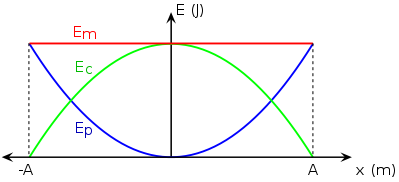
\includegraphics[width=0.5\linewidth]{Energia_MAS}
	\caption{Representación gráfica de $E_{m}$.}
	\label{fig:energiamas}
\end{figure}

\subsection{Reflexión y Refracción}
Una onda al encontrarse con otro medio puede ser reflectada de la siguiente forma:
\begin{figure}[h]
	\centering
	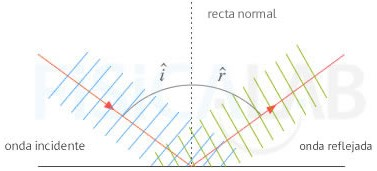
\includegraphics[width=0.4\linewidth]{onda-reflejada}
	\caption{$\hat{i}$ es el ángulo de la onda incidente con la recta normal y $\hat{r}$ de la reflejada con la normal.}
	\label{fig:onda-reflejada}
\end{figure}
Los ángulos $\theta_i$ y $\theta_r$ son iguales:
\begin{equation*}
	\hat{i}=\hat{r}\, \text{ o } \,\theta_i = \theta_r
\end{equation*}

Pero cuando la onda pasa al medio en el cual incide se da lugar una refracción:
\begin{figure}[h]
		\centering
		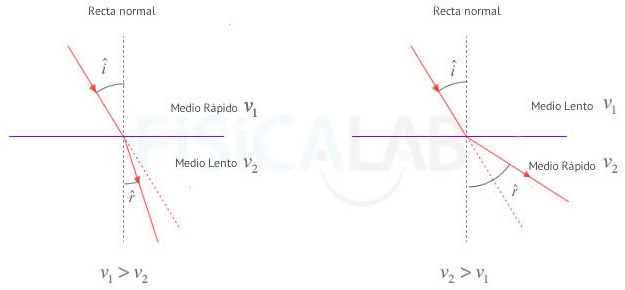
\includegraphics[width=.5\textwidth]{refraccion-ondas1}
		\caption{Se pueden ver las dos situaciones que dependen de la velocidad que tiene la onda en los medios.}
		\label{fig:refraccion1}
\end{figure}

Los ángulos en la figura anterior se describen mediante la ley de Snell\footnote{caracol}:
\begin{equation*}
	\frac{v_{1}}{v_{2}} = \frac{\sin\theta_i}{\sin\theta_r}
\end{equation*}
Existe el caso especial del ángulo limite:
\begin{equation*}
	\frac{v_{1}}{v_{2}} = \frac{\sin\theta_i}{\sin\frac\pi2} \Rightarrow \sin\theta_{lim} = \frac{v_{1}}{v_{2}}
\end{equation*} 
Cuando $v_{2} = v_{1}$, claro. Se ha de mencionar que cuando sucede este efecto la onda mantiene constante la frecuencia, pero al cambiar la velocidad de propagación, la longitud de onda cambia $\nu = \frac v\lambda$. 

También se tiene que tener claro el aspecto cualitativo de la difracción de una onda plana (figura \ref{fig:difraccion-ondas}). 
\begin{figure}[h]
	\centering
	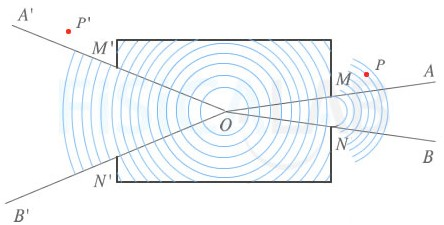
\includegraphics[width=0.5\linewidth]{difraccion-ondas}
	\caption{Difracción de una onda circular contenida dentro de una caja}
	\label{fig:difraccion-ondas}
\end{figure}

Se ha de tener en cuenta que mediante el principio de Huygens, los puntos en un frente de onda se comporta como emisores de esa onda. Se crean nuevos frentes con la misma frecuencia y velocidad de propagación. 


\subsection{Puntos máximos y mínimos en la interferencia de dos ondas}
Dos ondas de la misma frecuencia y longitud de onda cuando interfieren lo hacen de la siguiente manera:
\begin{align}
	A_{T} &= 2A\cos\left(k\frac{(x_{2}- x_{1})}{2} + \frac{(\varphi_1-\varphi_{2})}{2}\right) \\
	y_{T} &= y_1 + y_{2} \\
	y_{T} &= A_{T}\sin\left(\omega t - k\frac{(x_{1}-x_{2})}{2} + \frac{(\varphi_1+\varphi_2)}{2}\right) \\
	&= 2A\cos\left(k\frac{(x_{2}- x_{1})}{2} + \frac{(\varphi_1-\varphi_{2})}{2}\right)\sin\left(\omega t - k\frac{(x_{1}-x_{2})}{2} + \frac{(\varphi_1+\varphi_2)}{2}\right)\\
\end{align}
Donde los máximos y mínimos vienen dados por la ecuación (3) en la cual $x_{2} - x_{1}$ es la distancia entre los focos.

La interferencia se puede sacar a partir de una suma de cosenos o senos:
\begin{align*}
	\sin A + \sin B &= 2\sin\left(\frac{A+B}{2}\right)\cos\left(\frac{A-B}{2}\right) \\
	\cos A + \cos B &= 2\cos\left(\frac{A+B}{2}\right)\cos\left(\frac{A-B}{2}\right)
\end{align*}

\subsection{Onda estacionaria}
Cuando dos ondas de las mismas características pero que viajan en sentido contrario se superponen crean una onda estacionaria. Al ser una superposición con de ondas con la misma frecuencia, amplitud y fase, se representa con la siguiente suma:
\begin{equation*}
	y_{T} = y_{\text{indidente}} + y_{\text{reflectada}} = A\sin(\omega t -kx)-A\sin(\omega t + kx)
\end{equation*}
Aplicando una suma de senos tenemos que\footnote{También aplicamos $\sin-A = -\sin A$}:
\begin{equation*}
	y_{T} = 2A\cos(\omega t) \sin(-kx) = -2A\cos(\omega t)\sin(kx)
\end{equation*}

\pagebreak
Las ondas estacionarias forman armónicos: 
\begin{figure}[h]
	\centering
	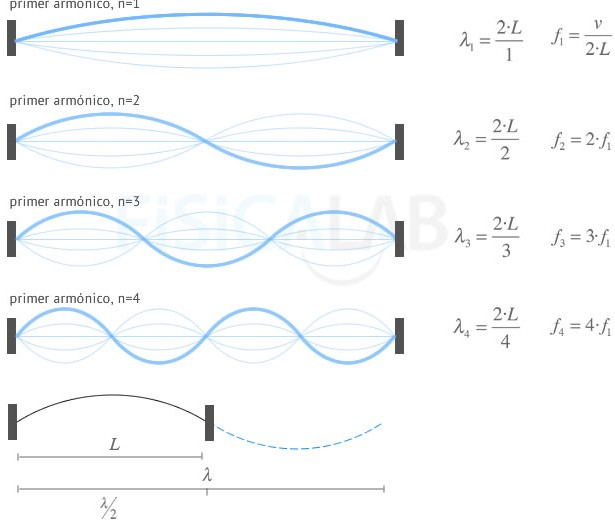
\includegraphics[width=0.6\linewidth]{onda-estacionaria-cuerda-fija}
	\caption{}
	\label{fig:onda-estacionaria-cuerda-fija}
\end{figure}
Donde el $n$ armónico contiene $n$ vientres i $n+1$ nodos y tiene una longitud de onda:
\begin{equation*}
	\lambda_{n} = \frac{2L}{n}
\end{equation*}
I por lo tanto una frecuencia $\nu_{n}$ ya que tienen que tener la misma velocidad:
\begin{align}
	v &= \lambda_{n}\nu_{n} \\
	\Rightarrow \nu_{n} &= \frac{v}{\lambda_{n}} = \frac{v}{\frac{2L}{n}} = n\frac{v}{2L}
\end{align}
Se ha de mencionar que las frecuencias de los armónicos, son múltiples de la frecuencia fundamental:
\begin{equation*}
	\nu_n = n\nu_1
\end{equation*}

Con las ondas con un extremo fijo el $n$-armónico es:
\begin{equation*}
	\lambda_{n} = \frac{4L}{2n-1}
\end{equation*}
Hay que remarcar que tendrá $n$ nodos y $n$ vientres.

En cambio, para las ondas con extremos libres:+
\begin{equation*}
	\lambda_{n} = \frac{2L}{n}
\end{equation*}
Y tendrá $n+1$ vientres y $n$ nodos. Aunque para todos los casos el número de vientres y nodos se puede saber en el momento.

Para saber la posición de los nodos en una onda estacionaria simplemente se tiene que utilizar la longitud total y $\lambda_{n}$. 

\subsection{Cualidades del sonido y intensidad}

Las cualidades del sonido son las siguientes:
\begin{enumerate}
	\item So: Es una onda mecánica que se propaga por diversos medios y puede ser detectada por el oído.
	\item Tono: Es la propiedad que define si un sonido en grave o agudo, está determinado cualitativamente por la frecuencia. 
	\item Timbre: Es la cualidad del sonido que define la forma de su onda. Depende de la fuente emisora. Un la de un piano y un violín son diferentes, ¿no?
\end{enumerate}

La intensidad de un sonido se mide mediante la potencia:
\begin{equation*}
	I =\frac PS = \frac 1S \dv{E}{t}
\end{equation*}
Para una onda 3D tenemos que:
\begin{equation*}
	I = \frac PS = \frac 1S \dv{E}{t} = \frac 1S\dv{t}\left[2\pi^{2}\rho\nu^{2}A^{2}V\right] = \frac{2\pi^{2}\rho\nu^{2}A^{2}}{S}\dv{V}{t}
\end{equation*}
En el caso de una onda esférica la superficie es $S=4\pi r^{2}$ y por lo tanto la intensidad es:
\begin{equation*}
	I = 2\pi^2\rho\nu^2A^{2}\dv{r}{t} = 2\pi^2\rho\nu^2A^{2}v
\end{equation*} 
Ja que el diferencial del radio es la velocidad $\dv{r}{t} = v$

Se ha definido en un nivel de intensidad sonora, el cual es una escala logarítmica que se mide en bel $\si{B}$:
\begin{equation*}
	\beta = \log\frac{I}{I_{o}}
\end{equation*}
Donde $I_{0} = 10^{-12} \si{Wm^{-2}}$ es la intensidad a la cual los humanos empiezan a oír.
Usualmente se trabaja con decibelios $\si{dB} = 10^1\si{B}$.

\subsection{Efecto Doppler}
Es un fenómeno que se da lugar cuando el emisor/receptor de una onda se desplaza respecto al otro.

Por ejemplo, cuando el foco se mueve hacia el receptor, el frente de la onda se comprime en esa dirección, por lo tanto, la longitud de onda disminuye y la frecuencia aumenta. Al mismo tiempo cuando se aleja el receptor, el frente de onda se separa y la frecuencia disminuye. Esto se puede pensar cualitativamente en el momento, para ello este tipo de diagramas pueden ayudar:
\begin{figure}[h]
	\centering
	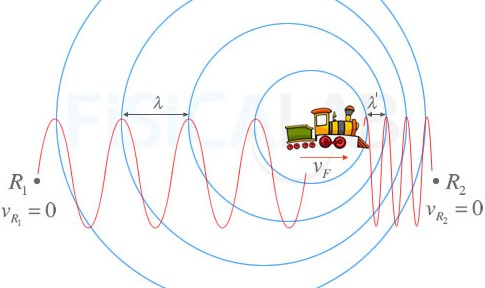
\includegraphics[width=0.5\linewidth]{efecto-doppler-2}
	\caption{Diagrama representativo del efecto Doppler con un tren moviéndose.}
	\label{fig:efecto-doppler-2}
\end{figure}

Este efecto se describe mediante la formula:
\begin{equation*}
	\nu' = \nu\frac{v\pm v_{O}}{v\mp v_{E}}
\end{equation*}
Donde $v_{O}$ es la velocidad del receptor y $v_{E}$ del emisor. 
No es necesario aprenderla pero si que se tiene que saber operar con ella. Normalmente se puede una explicación/interpretación del efecto. Si se ha de utilizar la formula, te la dan. 
\pagebreak

\section{Gravitación}
Los contenidos de este tema son menos, pero es importante tener en cuenta como se describe un movimiento circular, tanto uniforme como uniforme. Asimismo se ha de saber la Ley de Gravitación Universal y todas las leyes de Newton. 
\subsection{Leyes de Kepler}
Un punto importante de este tema son las leyes de Kepler:
\begin{enumerate}
	\item Los planetas giran alrededor del Sol describiendo órbitas elípticas en las cuales el sol es uno de los focos.
	\item Los planetas  giran alrededor del Sol con una velocidad areolar constante: En un tiempo determinado, el vector de posición define una área que es constante (figura \ref{fig:segunda-ley-kepler})\footnote{Área de un sector circular $A=\frac{\theta r^{2}}{2}$}.
	\item Los cuadrados de los períodos orbitales son directamente proporcionales a los semiejes más grandes de sus órbitas (la distancia más larga a la que están del sol): 
	\begin{equation*}
		\frac{T^2}{r^{3}} = \frac{{T'}^2}{{r'}^{3}}
	\end{equation*}
 	O alternativamente:
 	\begin{equation*}
 		\frac{r^{3}}{T^{2}} = G\frac{m_{\text{sol}}}{4\pi^{2}}
 	\end{equation*}
\end{enumerate}

\begin{figure}
	\centering
	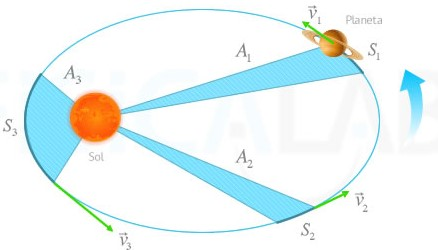
\includegraphics[width=0.5\linewidth]{segunda-ley-kepler}
	\caption{Tanto las velocidades ($ v_{1}, v_{2}, v_{3}$) como el recorrido del planeta en un tiempo determinado ($ S_{1}, S_{2}, S_{3}$) pueden ser diferentes entre si, pero las áreas siempre serán iguales $A_{1}=A_{2}=A_{3}$.}
	\label{fig:segunda-ley-kepler}
\end{figure}

Un aspecto importante es la deducción de la Tercera Ley de Kepler a partir de la Segunda Ley de Newton y la ley de la Gravitación Universal, si se pide será para un movimiento circular uniforme. 

Empezamos con la igualdad trivial de:
\begin{equation*}
	F = ma= G\frac{m_{1}m_{2}}{r^2}
\end{equation*}
Al describir un movimiento circular uniforme, podemos sustituir la aceleración por la aceleración centrípeta $a_{c}=\omega^2 r$\footnote{La ac. centrípeta es muy importante para deducir varios conceptos de este tema $ a_{c}= \omega^{2}r =  \frac{v^{2}}{r}$.}:
\begin{align*}
	m\omega^2r &= G\frac{m_{1}m_{2}}{r^2} \\
	m\left(\frac{2\pi}{T}\right)^{2} r&= G\frac{m_{1}m_{2}}{r^2}
\end{align*}
Se puede ver como $m=m^1$ ya que es la masa del objecto que órbita (entonces definimos $m_{2}$ como la masa del sol), al ser lo mismo se cancelan:
\begin{equation*}
	\left(\frac{2\pi}{T}\right)^{2} r = G\frac{m_{\text{sol}}}{r^2}
\end{equation*}
A continuación se puede aislar el periodo junto al radio para acabar con la Tercera Ley de Kepler:
\begin{equation*}
	\frac{r^{3}}{T^{2}} = G\frac{m_{\text{sol}}}{4\pi^{2}}
\end{equation*}

\subsection{Energía mecánica y tipos de órbitas}
Si la única fuerza actuando sobre un objecto en órbita es la fuerza gravitatoria, esta es igual a la centrípeta: 
\begin{equation*}
	G\frac{m_{1}m_{2}}{r^{2}} = m\frac{v^{2}}{r}
\end{equation*}
Por lo tanto la velocidad orbital es:
\begin{equation*}
	v=\sqrt{G\frac Mr}
\end{equation*}
Entonces se puede expresar la energía cinética como:
\begin{equation*}
	E_{k} = \frac 12 mv^2=\frac12m\left(G\frac Mr\right) = -\frac12 E_{p}
\end{equation*}
Donde $ E_{p}$ es la energía potencial gravitatoria:
\begin{equation*}
	E_{p} = -G\frac{m_{1}m_{2}}{r}
\end{equation*}
Finalmente tenemos que la energía mecánica es:
\begin{equation*}
	E_{m} = E_{k} + E_{p} = -\frac12E_{p} + E_{p} = \frac12 E_{p}
\end{equation*}

Es posible relacionar valores de energía mecánica a tipos de órbitas:
\begin{itemize}
	\item Negativa (Elíptica):\\
	Cuando la energía mecánica es positiva, el objecto describe una trayectoria elíptica o circular:
	\begin{figure}[h]
		\centering
		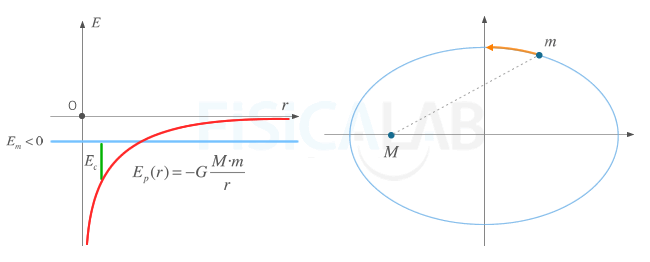
\includegraphics[width=0.6\linewidth]{energia-mecanica-negativa}
		\caption{Energía Negativa (Elíptica)}
		\label{fig:energia-mecanica-positiva}
	\end{figure}

	\item Nula (Parabólica):\\
	Cuando la energía mecánica es nula, el objecto describe una trayectoria parabólica:
	\begin{figure}[h]
		\centering
		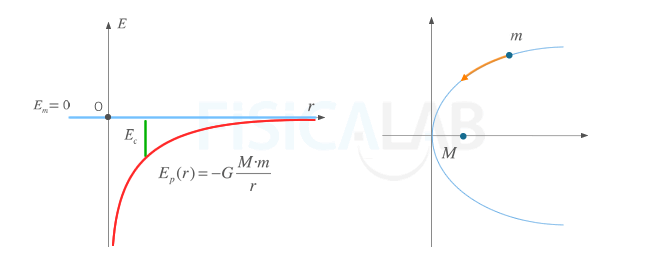
\includegraphics[width=0.6\linewidth]{energia-mecanica-nula}
		\caption{Energía Nula (Parabólica)}
		\label{fig:energia-mecanica-nula}
	\end{figure}

\pagebreak
	\item Positiva (Hiperbólica):\\
	Cuando la energía mecánica es negativa, el objeto describe una trayectoria hiperbólica:
	\begin{figure}[h]
		\centering
		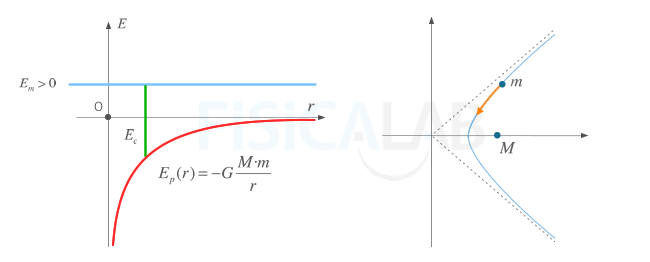
\includegraphics[width=0.6\linewidth]{energia-mecanica-positiva}
		\caption{Energía Positiva (Hiperbólica)}
		\label{fig:energia-mecanica-negativa}
	\end{figure}
\end{itemize}

Cabe remarcar que es el cambio de la energía mecánica es el que es nulo $\Delta E_{m}$, la energía en si misma no tiene porque serlo. También se puede referirse a ella como energía de enlace o energía mecánica orbital.

Conociendo la energía mecánica (a partir de la potencial), es posible definir una velocidad de escapamiento con la energía cinética, debido a que se ha de describir una trayectoria parabólica para escapar de la gravedad de un objecto:
\begin{align*}
	E_{m} &= 0 \\
	\frac12m_{1}v^2 - G\frac{m_{1}m_{2}}{r} &= 0  \\
	\Rightarrow v &= \sqrt{2G\frac{m_{2}}{r}}
\end{align*}
Donde $ v$ es la velocidad de escapamiento.

\section{Física moderna}
Este tema viene dividido en dos, una parte es la radioactividad (tiempo de desintegración y ecuaciones radioactivas) y la otra la física cuántica (efecto fotoeléctrico y energía asociada a las partículas). Siempre sale un ejercicio de cada uno de los subtemas.

\subsection{Ley de Desintegración Radioactiva}
Una muestra de material radioactivo se desintegra mediante su actividad radioactiva:
\begin{equation*}
	A = \dv{N}{t}
\end{equation*}
Podemos definirla mediante la ley de desintegración radioactiva:
\begin{equation*}
	\dv{N}{t} = -\lambda N
\end{equation*}
Donde $\lambda$ es la constante de desintegración y $N$ el número de isotopos.

La solución a esta ecuación es:
\begin{equation*}
	N = N_{0}e^{-\lambda t}
\end{equation*}
$N_{0}$ es la cantidad de material inicial y $N$ la cantidad de material que hay cuando pasa el tiempo $t$.

\subsection{Periodo de semidesintegración}
Se define el periodo de semidesintegración $t_{\frac12}$ como el tiempo que tarda una muestra radioactiva en reducirse a la mitad. Por la ley de desintegración sabemos que:
\begin{align*}
	\frac{1}{2} &= e^{-\lambda t_{\frac12}} \\
	\ln\frac12 &= -\lambda t_{\frac12}\\
	\Rightarrow t_{\frac12} &= -\frac{\ln\frac12}{\lambda} = \frac{\ln2}{\lambda}
\end{align*}
También se define la vida media $\tau$ de un isotopo como la inversa de la constante de desintegración:
\begin{equation*}
	\tau = \frac1\lambda
\end{equation*}

\subsection{Ecuaciones Radioactivas}
Un elemento $X$ se puede escribir como:
\begin{equation*}
	\ce{^Z_AX^{\pm n}}
\end{equation*}
Donde $\ce{Z}$ es el número de protones y neutrones, y $\ce{A}$ es el nombre atómico (número protones). $n$ sería la carga del elemento, en caso de que sea un ion, puede ser positiva o negativa. Esta notación también se aplica a partículas. 

Un ejemplo de ecuación radioactiva seria:
\begin{equation*}
	\ce{^216_{86}Rn -> ^4_2\alpha_ + ^212_84Po}
\end{equation*}
Se puede apreciar como la masa y la carga de los elementos y partículas se conserva. También en caso de que ho haya ningún tipo de radiación, el número de protones, neutrones y electrones se ha de conservar. Como ejemplo podemos completar la siguiente ecuación:
\begin{equation*}
	\ce{^{210}_{84}Po -> ^{x}_{y}Pb + ^{4}_{2}He}
\end{equation*}
Se ha de conservar el nombre atómico, por lo tanto:
\begin{equation*}
	84 = y + 2 \Rightarrow y = 84-2=82
\end{equation*}
Se ha de conservar el nombre massico, por lo tanto:
\begin{equation*}
	210 = x+ 4 \Rightarrow x = 210 -4=206
\end{equation*}

Hay 3 tipos de radiación, pero las que nos importa son la radiación beta, la cual se puede presentar de dos formas\footnote{Conviene memorizar el nombre de cada radiación dependiendo si contiene un electrón de carga negativa (la beta negativa) o de un positrón de carga positiva (la beta positiva).}, y la radiación alfa:
\begin{itemize}
	\item Radiación $\beta^{+}$ Positiva: \\
	Consiste en un protón que decae en un neutrón, positrón $\ce{e^+}$ y un neutrino electrónico $\ce{\nu_e}$:
	\begin{equation*}
		\ce{^{1}_{1}p^{+} -> ^{1}_{0}n^{0} + e^{+} + \nu_{e}}
	\end{equation*}

	\item Radiación $\beta^{-}$ Negativa: \\
	Consiste en un neutrón que decae en un protón, electrón $\ce{e^-}$ y un antineutrino electrónico $\ce{\nu_e}$:
	\begin{equation*}
		\ce{^{1}_{0}n^{0} -> ^{1}_{1}p^{+} + e^{-} + \overline{\nu_{e}}}
	\end{equation*}

	\item Radiación $\alpha$: \\
	Consisten un núcleo de helio:
	\begin{equation*}
		\ce{^{4}_{2}He}
	\end{equation*}
\end{itemize}

Cada radiación tiene un tipo de decaimiento, la manera en la que cambian los elementos que liberan las partículas correspondientes a cada radiación:
\begin{itemize}
	\item Decaimiento $\beta^{-}$: \\
	\begin{equation*}
		\ce{\beta^{-} \colon^Z_AX -> ^Z_{A+1}Y + e^{-} + \overline{\nu_{e}}}
	\end{equation*}
	
	\item Decaimiento $\beta^{+}$: \\
	\begin{equation*}
		\ce{\beta^{+}\colon ^A_ZX -> ^A_{Z-1}Y + e^{+} + \nu_{e}}
	\end{equation*}

	\item Decaimiento $\alpha$: \\
	\begin{equation*}
		\ce{^Z_{A}X -> ^4_2\alpha_ + ^{Z-4}_{A-2}Po}
	\end{equation*}
\end{itemize}

\subsection{Efecto fotoeléctrico}
Es un fenómeno que surge cuando se irradia con radiación electromagnética y genera una corriente (flujo electrones) en un mental. Cuando se irradia el metal este desprende electrones, formando un flujo. 

Si hay un aumento de la frecuencia de la radiación, aumenta la energía cinética de los electrones. Es cuando hay un aumento de la intensidad luminosa que es cuando hay un aumento del flujo de electrones. 

Este efecto se describe mediante la ecuación:
\begin{align*}
	E = h\nu &= E_{i} + E_{k} \\
	&= h\nu_0 + \frac12mv^2 
\end{align*}
Donde $E$ es la energía del fotón, $E_{i}$ la energía de ionización (energía necesaria para arrancar un electrón de un átomo) y $E_{k}$ es la energía cinética del electrón. Se puede ver como cuando $E$ sobrepasa $E_{i}$ es cuando existe una $E_{k}$ y por lo tanto el fotón es arrancado. Realmente solo la energía cinética es la que cambia con la frecuencia del fotón porque la energía de ionización se queda constante. 

Normalmente se da una frecuencia lindar para hacer cálculos con esta ecuación, $E_{i}$ seria la energía asociada a esta frecuencia. 

\subsection{Dependencia de la masa según la velocidad}
Según la relatividad especial una masa varia a partir de la velocidad de acuerdo con la ecuación:
\begin{equation*}
	m=m_{0}\gamma
\end{equation*}
Donde $\gamma$ es el factor gamma:
\begin{equation*}
	\gamma = \frac{1}{\sqrt{1-\frac{v^2}{c^{2}}}} = \frac{c}{\sqrt{c^{2} - v^2}}
\end{equation*}
Normalmente simplemente se escribe como:
\begin{equation*}
	m=\frac{1}{\sqrt{1-\frac{v^2}{c^{2}}}}m_{0}
\end{equation*}

También se pueden referir a esto no sé:
\begin{equation*}
	E^{2} = p^{2}c^{2} + m_{0}^{2}c^{4}
\end{equation*}

\subsection{Principio de incertidumbre de Heisenberg}
Como ya sabemos existen magnitudes observables en la física como la posición o la velocidad, las cuales se pueden definir perfectamente observando un objecto en un tiempo determinado. Pero en mecánica cuántica se aplica el principio de incertidumbre de Heisenberg que esmenta que estas magnitudes están conjugadas. Esto quiere decir que no se pueden observar con presión para una determinada partícula en un determinado momento en el tiempo. Cuando se mide con presión la velocidad, la masa queda indeterminada. Esto también sucede al contrario. 

La ecuación que cuantifica este principio es la siguiente\footnote{$\hslash = \frac{h}{2\pi}$}:
\begin{equation*}
	\Delta x\Delta p \geq \frac{h}{4\pi} = \frac{\hslash}{2}
\end{equation*}
Donde $\Delta x$ i $\Delta p$ son la impresición en la posición i el momento respectivamente.

\pagebreak
\section{Campo eléctrico}

\subsection{Energía, Campo Eléctrico, Potencial, Fuerza Eléctrica}
Un campo electrónico creado por una distribución de cargas se define como:
\begin{equation*}
	\overrightarrow{E} = \sum^{n}_{i=1}\frac{1}{4\pi\varepsilon_{0}}\frac{q_{i}}{r^{2}_{i}}\hat{r}_{i}
\end{equation*} 
Donde una carga $q_{i}$ está a una distancia $r_{i}$ definida por un vector de posición $\hat{r}_{i}$.

Asimismo la fuerza entre una distribución de cargas sobre una carga $q$ es:
\begin{equation*}
	\overrightarrow{F} = \sum_{i=1}^{n}\frac{1}{4\pi\varepsilon_{0}}\frac{qq_{i}}{r^{2}_{i}}\hat{r}_{i}
\end{equation*}

Se puede ver como el campo eléctrico, es la fuerza magnética dividida por la carga a la cual se aplica la fuerza:
\begin{equation*}
	\overrightarrow{E} = \frac{\overrightarrow{F}}{q} = \frac{1}{4\pi\varepsilon_{0}} \frac{q}{r^{2}}\hat{r} = k\frac{q}{r^2}\hat{r}
\end{equation*}
Por el contrario también es verdad que:
\begin{equation*}
	\overrightarrow{F} = q\overrightarrow{E}
\end{equation*}

Además se puede definir un potencial eléctrico creado por una distribución de cargas a partir de la energía potencial eléctrica:
\begin{equation*}
	V(r) = \frac{E_{p}(r)}{q'} = k\frac{qq'}{rq'} = k\frac{q}{r}
\end{equation*} 
Se puede ver como la energía potencial es\footnote{Energía potencial de una carga $q'$ en el campo magnético creado por una carga $q$.}:
\begin{equation*}
	E_{p}(r)=k\frac{qq'}{r}
\end{equation*}
Añadiendo la energía cinética podemos definir una energía mecánica que ha de ser constante ($\Delta E_{m} = 0$):
\begin{equation*}
	E_{m} = E_{k} + E_{p} = \frac12 mv^{2} + k\frac{qq'}{r}
\end{equation*}

También es importante saber la relación entre el campo eléctrico y el potencial eléctrico: Un campo eléctrico siempre apunto en la dirección en que el potencial decrece. Esto se pueden expresar fácilmente con una derivada:
\begin{equation*}
	E = -\dv{V}{x}\,\text{ o alternativamente }\, \overrightarrow{E} = -\dv{V}{x}\hat{i}
\end{equation*}

Asimismo el potencial también se puede relacionar con la energía potencial simplemente multiplicando por una carga:
\begin{equation*}
	\Delta E_{p} = q'\Delta V
\end{equation*}

\pagebreak
\subsection{Diagramas de líneas de campo}
Un ejemplo de un diagrama de líneas de campo es el siguiente:
\begin{figure}[h]
	\centering
	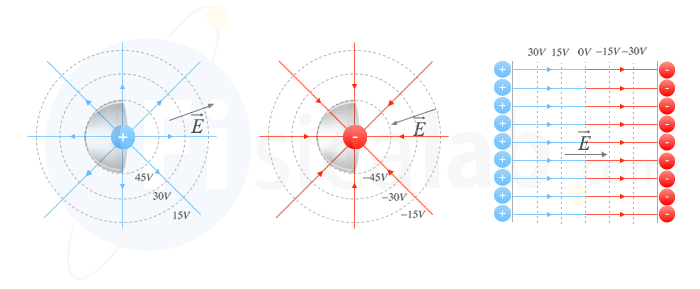
\includegraphics[width=0.6\linewidth]{potencial-e-intensidad}
	\caption{Diagrama de movimiento de cargas en un campo eléctrico}
	\label{fig:potencial-e-intensidad}
\end{figure}
Donde las líneas discontinuas son las líneas equipotenciales, donde todos los puntos sobre ellas tienen el mismo potencial, ya que están a la misma distancia de la carga. Se puede ver como en la tercera hay una diferencia de potencial entre un grupo de cargas, y que el campo eléctrico circula de positivo a negativo. Las líneas de campo siempre salen de una carga positiva y entran en una carga negativa.

\subsection{Movimiento de una carga a través de un campo eléctrico}
Una carga siempre se moverá siguiendo la fuerza electrostática, es decir la carga multiplicada por el campo eléctrico:
\begin{equation*}
	\overrightarrow{F}_{e} = q\overrightarrow{E}
\end{equation*}
Hay que tener en cuenta que una carga positiva se mueve en el sentido del campo eléctrico, y una negativa al contrario. También se pueden entender esto como que la carga se mueve en el sentido del potencial (el cual tiene signo). 

\subsection{Onda electromagnética}
Es lo mismo que las ondas armónicas planas pero solo que son ondulaciones en el campo eléctrico y magnético que son perpendiculares entre si y suceden al mismo tiempo:
\begin{figure}[h]
	\centering
	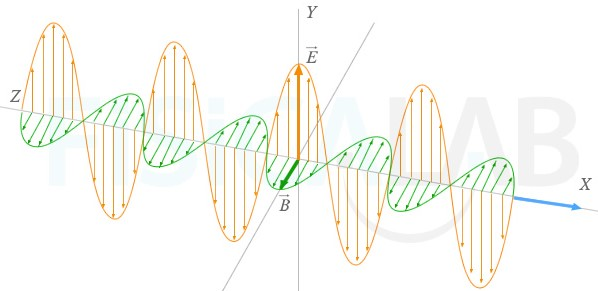
\includegraphics[width=0.4\linewidth]{sintesis-electromagnetica}
	\caption{Onda electromagnética}
	\label{fig:sintesis-electromagnetica}
\end{figure}
\\
La dirección de propagación de una onda viene definida por el producto vectorial de los campos:
\begin{equation*}
	\overrightarrow{S} = \frac{\overrightarrow{E}\cross\overrightarrow{B}}{\mu}
\end{equation*}
También cabe destacar que tiene propiedades como la polarización y puede ser absorbida o reflectada. 


\section{Electromagnetismo}
\subsection{Fuerza sobre conductores rectilíneos debajo de la acción de un campo magnético}
Si tenemos un hilo conductor de longitud $L$ y por el cual circula una corriente $I$, la fuerza magnética de $N$ portadores de carga se puede expresar como:
\begin{equation*}
	\overrightarrow{F}_{m} = Nq(\overrightarrow{v}\cross\overrightarrow{B}) = Nq\left(\frac{\overrightarrow{L}}{\Delta t}\cross\overrightarrow{B}\right) = \frac{Nq}{\Delta t}\overrightarrow{L}\cross\overrightarrow{B}
\end{equation*}
Debido a que se $\frac{Nq}{\Delta t}$ es la Intensidad de la corriente, la fuerza se puede escribir como:
\begin{equation*}
	\overrightarrow{F}_{m} = I\overrightarrow{L}\cross\overrightarrow{B}
\end{equation*}

\subsection{Inducción campo magnético}
\subsubsection{Conductor rectilíneo}
Un conductor rectilíneo por el cual circula una corriente $I$, genera un campo magnético de intensidad:
\begin{equation*}
	B=\frac{\mu}{2\pi}\frac{I}{d}
\end{equation*}
Donde $d$ es la distancia a la cual se encuentra el punto que tiene esa intensidad. 

Utilizando la regla de la mano derecha se puede ver como los dedos indican el sentido del campo circular que se genera:
\begin{figure}[h]
	\centering
	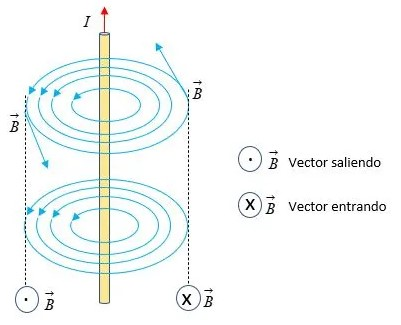
\includegraphics[width=0.5\linewidth]{magnetico_linea}
	\caption{Campo magnético generado por un conductor rectilíneo}
	\label{fig:magneticolinea}
\end{figure}
(el pulgar tiene que ir en la dirección y sentido de la intensidad)

\subsubsection{Espira}
Asimismo una espira circular genera un campo magnético en su centro su centro dependiendo de su radio $R$ y intensidad:
\begin{equation*}
	B_{\text{centro}} = \frac{\mu I}{2R}
\end{equation*}
Cuando hay $N$ juntas la intensidad se multiplica por $M$:
\begin{equation*}
	B_{\text{centro}} = NB_{\text{espira}} = \frac{N\mu I}{2R}
\end{equation*}

\subsubsection{Solenoide}
Si se colocan varias espiras unidas, por las cuales circula una corriente se obtiene un solenoide, el cual es su eje tiene una intensidad de campo magnético inducido de:
\begin{equation*}
	B_{\text{int}} = \frac{\mu NI}{L} = \mu nI
\end{equation*}
Donde $n=\frac{N}{L}$ es la densidad de espiras. 

\begin{figure}
	\centering
	\hfill
	\begin{subfigure}[b]{0.5\textwidth}
		\centering
		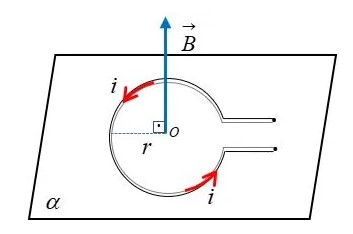
\includegraphics[width=\textwidth]{espira}
		\caption{Campo magnético inducido por una espira}
		\label{fig:espira}
	\end{subfigure}
	\hfill
	\begin{subfigure}[b]{0.25\textwidth}
		\centering
		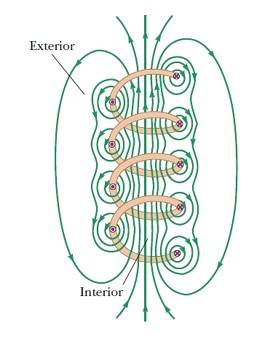
\includegraphics[width=\textwidth]{solenoide}
		\caption{Campo magnético inducido por un solenoide}
		\label{fig:five over x}
	\end{subfigure}
	\caption{}
	\label{fig:solenoide}
\end{figure}

\subsection{Fuerza magnética sobre una carga}
La fuerza de Lorentz describe la fuerza magnética sobre una carga que ubica cobre un campo magnético:
\begin{equation*}
	\overrightarrow{F}_{m} = q(\overrightarrow{v}\cross\overrightarrow{B})
\end{equation*}
A través de la definición del producto vectorial podemos ver que:
\begin{equation*}
	F_{m} = qvB\sin\theta 
\end{equation*}
Donde $\theta$ es el angulo entre el vector de la velocidad y el campo magnético sobre un plano.
Entonces si la velocidad y el campo son ortogonales entre si la intensidad será simplemente $F_{m}=qvB$. 

Podemos generalizar esta ecuación considerando la existencia de un campo eléctrico:
\begin{equation*}
	\overrightarrow{F} = q(\overrightarrow{E} + \overrightarrow{v}\cross\overrightarrow{B})
\end{equation*}

También se puede ver como solo existe la fuerza en caso de que la carga entre en movimiento.

En caso de que sean perpendicular la carga comenzará a describir un movimiento circular:
\begin{equation*}
	qvB=m\frac{v^{2}}{R}
\end{equation*}
Por lo tanto, el radio de la trayectoria es:
\begin{equation*}
	R=\frac{mv}{qB} = \frac{p}{qB}
\end{equation*}

\subsection{Flujo magnético y fuerza electromotriz}

El flujo magnético es una magnitud que cuantifica la cantidad de líneas de campo que atraviesa una determinada superficie:
\begin{equation*}
	\Phi = \overrightarrow{B}\cdot\overrightarrow{S} = BS\cos\theta
\end{equation*}
Se calcula a partir del producto escalar entre el vector que define el campo magnético y el vector que define la superficie que atraviesa el campo. Se puede simplificar mediante el coseno del angulo entre el vector del campo y el vector normal de la superficie. 

Al derivar el flujo magnético sobre el tiempo se llega a la fuerza electromotriz:
\begin{equation*}
	\varepsilon(t) = -\dv{\Phi(t)}{t}
\end{equation*}
En caso de que sean una superficie variable (que se mueve) la fuerza electromotriz depende de su velocidad:
\begin{equation*}
	\varepsilon = -\dv{\Phi(t)}{t} = -BLv
\end{equation*}
Donde $L$ es una magnitud que describe longitud, ¿de qué?, pues no lo sé. 


\end{document}
